
\documentclass{beamer}
\usepackage{amssymb}
\usepackage{stackengine}
\usepackage{beamerthemeshadow}
\newcommand\stackrqarrow[2]{%
	\mathrel{\stackunder[2pt]{\stackon[4pt]{$\rightsquigarrow$}{$\scriptscriptstyle#1$}}{%
			$\scriptscriptstyle#2$}}}
\begin{document}
\title{Algoritmi pentru grafuri \c si aplica\c tii}  
\author{G\u albini\c t\u a Sebastian}
\date{\today} 

\frame{\titlepage} 

\frame{\frametitle{Cuprins}\tableofcontents} 


\section{Drumuri minime de surs\u a unic\u a} 
\frame{\frametitle{Drumuri minime de surs\u a unic\u a} 
 Fie un graf orientat ponderat $G=(V,E)$ \c si func\c tia cost $f:E \longrightarrow \mathbb{R}$. \textbf{Costul} drumului  $p=[ \alpha_{0},\alpha_{1},....,\alpha_{k}]$ este dat de
     \begin{equation*}
 f(p)=\sum\limits_{i=1}^{k} f(\alpha_{i-1},\alpha_{i})
 \end{equation*}
 Astfel putem defini \textbf{costul unui drum minim}
   	\begin{equation*}
 \delta(u,v)=
 \begin{cases}
 min\left\{f(p):u\leadsto v\right\},&\text{dac\u a exist\u a drum de la $u$ la $v$} \medskip\\
 \infty,& \text{altfel} \medskip
 \end{cases}
 \end{equation*} 
}
\subsection{Relaxare }

\frame[plain]{ \frametitle{Relaxare}
	Pentru fiecare nod $v\in V$, se va re\c tine un \textbf{predecesor} $\omega[v]$ \c si conserv\u am un atribut $d[v]$.
	
	
	Procesul de relaxare a unei muchii $(u,v)$  este dat de urm\u atoarea inegalititate:
	\begin{equation*}
	d[v]>d[u]+f(u,v)
	\end{equation*}
	
 \begin{figure}[!hbt]
	\centering
	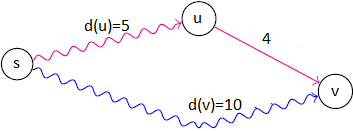
\includegraphics[width=6cm]{Relaxeaza.png}
	
\end{figure}
}
\subsection{Algoritmul lui Dijkstra}
\frame[plain]{\frametitle{Algoritmul lui Dijkstra}
	Algoritmul lui Dijkstra rezolv\u a problema drumurilor minime de surs\u a unic\u a \^ intr-un graf orientat ponderat $G=(V,E)$ pentru care toate costurile muchiilor sunt nenegative. Vom presupune c\u a pentru fiecare muchie $(u,v)\in E$, $f(u,v)\geq 0$.
	
	
    \vspace{0.3cm}
DIJKSTRA $(G,f,s)$

\vspace{0.1cm}
1: INI\c TIALIZEAZ\u A-SURS\u A-UNIC\u A$(G,s)$

2: $S\longleftarrow \emptyset$  

3: $Q\longleftarrow V(G)$

4: \textbf{while} $Q\ne \emptyset$ 

5:\hspace{0.6cm} $u\longleftarrow$ EXTRAGE-MIN(Q)

6:\hspace{0.6cm} $S\longleftarrow S\cup \{u\}$

7:\hspace{0.6cm} \textbf{for} fiecare v\^ arf $v\in Adj[u]$

8:\hspace{1.2cm} RELAXEAZ\u A$(u,v,f)$
\vspace{0.3cm}
}


\section{Drumuri minime \^ intre toate perechile de v\^ arfuri} 
\frame{\frametitle{Drumuri minime \^ intre toate perechile de v\^ arfuri}
 Fie un graf orientat ponderat $G=(V,E)$ \c si o func\c tie de costuri  $f:E \longrightarrow \mathbb{R}$ aplicat\u a arcelor grafului. 
 Pentru fiecare $u,v\in V$, determin\u am un \textbf{drum de cost minim} de la $u$ la $v$. Ca date de intrare avem o matrice A, av\^ and dimensiunea $n\times n$.
 
  \begin{equation*}
 a_{ij}=
 \begin{cases}
 0,&\text{dac\u a $i=j$}, \medskip\\
 f(i,j),& \text{dac\u a $i\ne j$ \c si $(i,j)\in E$}, \medskip\\
 \infty,&\text{dac\u a $i\ne j$ \c si $(i,j)\notin E$}.\medskip
 \end{cases}
      \end{equation*}
        Iar ca date de ie\c sire o matrice $D=(d_{ij})$ de dimensiune $n\times n$. 
}
\subsection{Structura unui drum minim}
\frame[plain]{\frametitle{Structura unui drum minim}
 Presupunem c\u a graful este reprezentat printr-o matrice de adiacen\c t\u a $A=(a_{ij})$. Consider\u am un \textbf{drum minim} $p$ de la nodul $i$ la $j$ \c si presunem c\u a are $m$ arce. Presupun\^ and c\u a  nu sunt cicluri de cost negativ, atunci $m$ este finit. Dac\u a $i=j$, atunci $p$ are costul 0 \c si nu con\c tine nici un arc. Dac\u a nodurile sunt distincte, atunci descompunem drumul $p$ \^ in  $i\stackrqarrow{p'}{ } k\rightarrow j$, unde drumul $p'$ con\c tine  cel mult $m-1$ arce. Mai mult, $p'$ este un drum minim de la $i$ la $k$. Deci avem urm\u atoarea egalitate:
      \begin{equation*}
 \delta (i,j)=\delta (i,k)+f(k,j).
 \end{equation*}
}
\frame[plain]{\frametitle{Determinarea drumurilor minime}
	Presupunem ca date de intrare matricea $A=(a_{ij})$, determin\u am o serie de matrici $D^{(1)},D^{(2)},...,D^{(n-1)}$, unde, pentru $m=1,2,...,n-1$ avem $D^{(m)}=(d_{ij}^{(m)})$. Matricea final\u a $D^{(n-1)}$ va con\c tine costurile drumurilor minime.
	
	 \vspace{0.3cm}
	
	     \vspace{0.3cm}
	EXTINDE$(D,A)$
	
	\vspace{0.1cm}
	1: $n\leftarrow linii[D]$
	
	2: fie $B=(b_{ij})$ matrice cu dimensiunea $n\times n$ 
	
	3: \textbf{for} $i\leftarrow 1,n$ 
	
	4: \hspace{0.6cm}\textbf{for} $j\leftarrow 1,n$ 
	
	5:\hspace{1.2cm} $b_{ij}\leftarrow \infty$
	
	6:\hspace{1.2cm} \textbf{for} $k\leftarrow 1,n$ 
	
	7:\hspace{1.8cm} $b_{ij}\leftarrow $min$(b_{ij},d_{ik}+a_{kj})$
	
	8: \textbf{return} B
	\vspace{0.3cm}
	
	
	
}
\frame[plain]{\frametitle{Determinarea drumurilor minime}
		 \begin{equation*}
	d_{ij}^{(m)}=\text{min} \bigg( d_{ij}^{(m-1)},\min_{1\leq k \leq n} \bigg\{  d_{ik}^{(m-1)}+a_{kj}\bigg\} \bigg) = \min_{1\leq k \leq n}\bigg\{  d_{ik}^{(m-1)}+a_{kj}\bigg\}
	\end{equation*}
	
	Deoarece am determinat \c sirul de $n-1$ matrice, putem transpune tot ce scris 
	\^ intr-o func\c tie.
		 \vspace{0.3cm}
	
	\vspace{0.3cm}
	
		DRUMURI-MINIME$(A)$
	
	\vspace{0.1cm}
	1: $n\leftarrow linii[A]$
	
	2: $D^{(1)}\leftarrow A $
	
	3: \textbf{for} $i\leftarrow 2,n-1$ 
	
	4: \hspace{0.6cm} $D^{(i)}\leftarrow $EXTINDE ($D^{(i-1)},A$)
	
	5: \textbf{return} $D^{(n-1)}$
	\vspace{0.3cm}
}
\subsection{Algoritmul Floyd-Warshall}
\frame{\frametitle{Algoritmul Floyd-Warshall}
 Algoritmul lui Floyd-Warshall este un algoritm pentru g\u asirea celor mai scurte drumuri \^ intr-un graf orientat ponderat cu cost pozitiv sau negativ. Acest algoritm se bazeaz\u a pe urm\u atoarea observa\c tie. 
 
 Fie $V=\{1,2,...,n\}$ mul\c timea nodurilor lui $G$. Consider\u am submul\c timea $\{1,2,...,k\}$ pentru un anumit $k$. Pentru orice pereche de noduri $i,j\in V$, consider\u am toate drumurile de la $i$ la $j$ ale c\u aror noduri intermediare fac parte din mul\c timea $\{1,2,...,k\}$. Fie $p$ drumul de cost minim dintre aceste drumuri. Algoritmul Floyd-Warshall exploateaz\u a o rela\c tie \^ intre drumul $p$ \c si drumul minim de la $i$ la $j$ cu toate nodurile intermediare.
}\frame[plain]{
\vspace{0.5cm}	
\hspace{1.6cm} {\scriptsize	toate nodurile intermediare \hspace{0.5cm} toate nodurile intermediare 
	
	\hspace{1.6cm}	din  $\{1,2,...,k-1\}$  \hspace{1.7cm}	din  $\{1,2,...,k-1\}$}
 \begin{figure}[!hbt]
	\centering
	\hspace{0.5cm}
	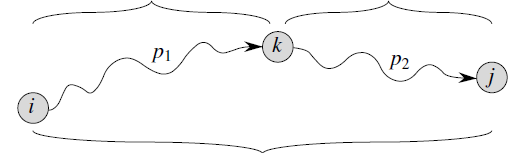
\includegraphics[width=7.2cm,height=2cm]{Warshall.png}
	\newline
	{\scriptsize $p$: toate nodurile intermediare din $\{1,2,...,k\}$}
	
\end{figure}
Dac\u a $k$ nu este nod intermediar al drumului $p$, un drum minim de la nodul $i$ la $j$ cu toate nodurile intermediare din mul\c timea $\{1,2,...,k-1\}$ este, de asemenea, un drum minim de la $i$ la $j$  cu toate nodurile intermediare din mul\c timea $\{1,2,...,k\}$.

Dac\u a $k$ este nod intermediar al drumului $p$, atunci  \^ imp\u ar\c tim $p$ \^ in dou\u a alte drumuri. Deoarece $p$ este drum minim rezult\u a c\u a \c si $p_1$ este drum minim de la $i$ la $k$ cu toate nodurile intermediare din mul\c timea $\{1,2,...,k-1\}$. Analog pentru $p_2$.
}
\frame[plain]{
	
	Intrarea este o matrice $A$ de dimensiune $n\times n$. Func\c tia returneaz\u a matricea $D^{(n)}$ a costurilor drumurilor minime.
		 \vspace{0.3cm}

\vspace{0.3cm}

FLOYD-WARSHALL$(A)$

\vspace{0.1cm}
1: $n\leftarrow linii[A]$

2: $D^{(0)}\leftarrow A $

3: \textbf{for} $k\leftarrow 1,n$ 

4: \hspace{0.6cm}\textbf{for} $i\leftarrow 1,n$ 

5: \hspace{1.2cm}\textbf{for} $j\leftarrow 1,n$ 

6:\hspace{1.8cm} $d_{ij}^{(k)}\leftarrow min\big(d_{ij}^{(k-1)},d_{ik}^{(k-1)}+d_{kj}^{(k-1)})$

7: \textbf{return} $D^{(n)}$
\vspace{0.3cm}
}

\section{Flux maxim} 
\frame{\frametitle{Flux maxim}
	Problema \textbf{fluxului maxim} este aceea de a determina cantitatea cea mai mare de material care poate fi transportat\u a pornind de la surs\u a \c si ajung\^ and la destina\c tie \c tin\^ and cont de restric\c tiile de capacitate.
	
	 \begin{figure}[!hbt]
		\centering
		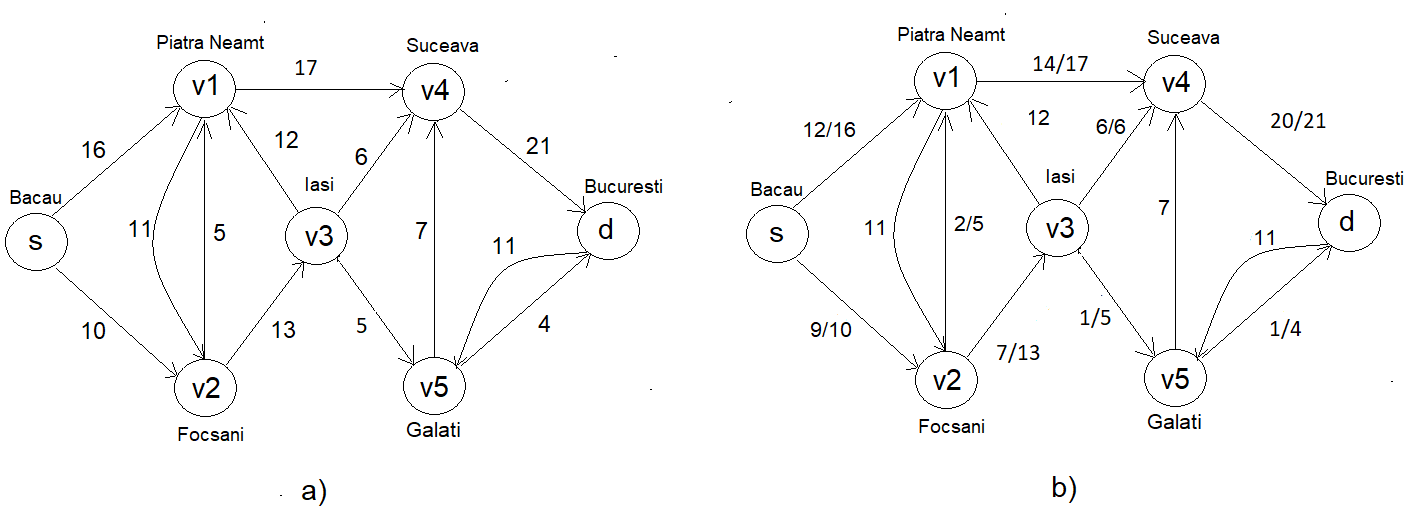
\includegraphics[width=10cm]{Flux.png}

	\end{figure}
}

\frame[plain]{\frametitle{Fluxuri \c si re\c tele de transport}
	O \textbf{re\c tea de transport} este un graf orientat $G=(V,E)$ \^ in care fiec\u arei muchii $(u,v)\in E$ \^ ii este ata\c sat\u a o \textbf{capacitate} nenegativ\u a $c(u,v)\geq 0$. Dac\u a $(u,v)\notin E$ atunci consider\u am $c(u,v)=0$. Fix\u am nodul surs\u a $s$ \c si nodul destina\c tie $d$. Denumim \textbf{fluxul} $G$ ca fiind o func\c tie $f:V\times V\rightarrow \mathbb{R}$ care satisface urm\u atoarele condi\c tii:
	\begin{enumerate}
		\item \textbf{Restric\c tia de capacitate}: Pentru orice $u,v\in V$, $f(u,v)\leq c(u,v)$.
		\item \textbf{Antisimetria}: Pentru orice $u,v\in V$,$f(u,v)=-f(u,v)$.
		\item \textbf{Conservarea fluxului}: Pentru orice $u\in V\setminus \{s,d\}$ avem
		 		\begin{equation*}
		\sum\limits_{v\in V} f(u,v)=0
		\end{equation*}
	\end{enumerate}

    Denumim \textbf{capacitatea rezidual\u a} a arcului $(u,v)$ ca fiind cantitatea de flux adi\c tional\u a care poate fi transportat\u a de la $u$ la $v$, f\u ar\u a a dep\u a\c si $c(u,v)$.
}


\subsection{Metoda lui Ford-Fulkerson}
\frame{\frametitle{Metoda lui Ford-Fulkerson}
	\^ In fiecare itera\c tie a metodei lui Ford-Fulkerson c\u aut\u am un drum \textit{oarecare} de ameliorare $p$ \c si m\u arim fluxul $f$ de-a lungul drumului $p$ cu capacitatea rezidual\u a $c_{f}(p)$.
	
	   	\vspace{0.3cm}
	METODA-FORD-FULKERSON$(s,d,G)$  	
	\vspace{0.1cm}
	
	1: \textbf{for} fiecare arc $(u,v)\in E[G]$ 
	
	2: \hspace{0.6cm} $f(u,v)\leftarrow 0$
	
	3: \hspace{0.6cm} $f(v,u)\leftarrow 0$
	
	4: \textbf{while} exist\u a un drum de la $s$ la $d$  \^ in re\c teaua rezidual\u a $G_f$ 
	
	5: \hspace{0.6cm} $c_f(p)\leftarrow min\{c_f(u,v)|(u,v)\in p\}$
	
	6: \hspace{0.6cm} \textbf{for} fiecare $(u,v)$ din $p$ 
	
	7:\hspace{1.2cm} $f(u,v)\leftarrow f(u,v)+c_f(p)$
	
	8:\hspace{1.2cm} $f(u,v)\leftarrow -f(u,v)$
	\vspace{0.3cm}
}
\section{Aplica\c tie}

\end{document}

